\documentclass{beamer}
\usepackage[orientation=portrait,size=a2,scale=1.4,debug]{beamerposter}
\mode<presentation>{\usetheme{ZH}}
\usepackage{chemformula}
\usepackage[utf8]{inputenc}
\usepackage[german, english]{babel} % required for rendering German special characters
\usepackage{siunitx} %pretty measurement unit rendering
\usepackage{hyperref} %enable hyperlink for urls
\usepackage{ragged2e}
\usepackage{subcaption}
\usepackage{amsmath}
\usepackage{amssymb}
\usepackage{sansmathaccent}
\pdfmapfile{+sansmathaccent.map}

%\usepackage[font=scriptsie,justification=justified]{caption}
\usepackage{array,booktabs,tabularx}

\newcolumntype{Z}{>{\centering\arraybackslash}X} % centered tabularx columns
\sisetup{per=frac,fraction=sfrac}

\title{\huge Graph matching with lobsters}
\author{Author: Sizhe Yuen \\[0.5ex] Supervisor: Kasim Terzi\'{c}}
\institute[ETH]{School of Computer Science, University of St Andrews}
\date{\today}

% edit this depending on how tall your header is. We should make this scaling automatic :-/
\newlength{\columnheight}
\setlength{\columnheight}{104cm}

\begin{document}
\begin{frame}
\begin{columns}

% Left columns
\begin{column}{.4\textwidth}
\begin{beamercolorbox}[center]{postercolumn}
\begin{minipage}{.98\textwidth}  % tweaks the width, makes a new \textwidth
\parbox[t][\columnheight]{\textwidth}{ % must be some better way to set the the height, width and textwidth simultaneously


\begin{myblock}{Abstract}
The ability to make measurements on lobsters is important in monitoring the size and health of the creatures.
This project explores the representation of lobsters as attributed graphs to discover and measure properties such as their size, using an existing dataset of lobster images.
Computer vision techniques are applied to detect interest points of different lobster body parts. 
Probabilistic models and subgraph matching are then used to label and build up the graph representation.
\end{myblock}


\begin{myblock}{Keypoint detection}
Different feature detection algorithms were tried to see which would provide useful keypoints consistently.

\begin{center}

\begin{minipage}{0.42\textwidth}
\begin{figure}
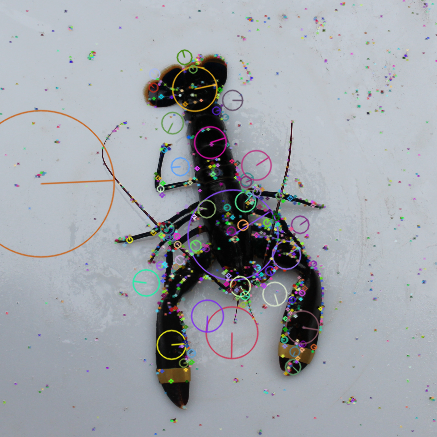
\includegraphics[width=1\textwidth, keepaspectratio]{imgs/sift.png}
\caption{SIFT detector}
\end{figure}
\end{minipage}
\hspace{0.7cm}
\begin{minipage}{0.42\textwidth}
\begin{figure}
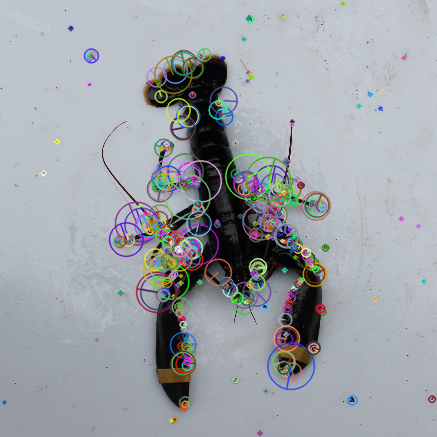
\includegraphics[width=1\textwidth, keepaspectratio]{imgs/surf.png}
\caption{SURF detector}
\end{figure}
\end{minipage}
\end{center}
\vspace*{-0.5cm}
\end{myblock}

\begin{myblock}{Keypoint filtering}
Multiple methods had to be used to filter out irrelevant keypoints. Octave filtering removed small keypoints and colour histogram filtering removed keypoints not on the lobster.
\begin{center}
\begin{minipage}{0.42\textwidth}
\begin{figure}
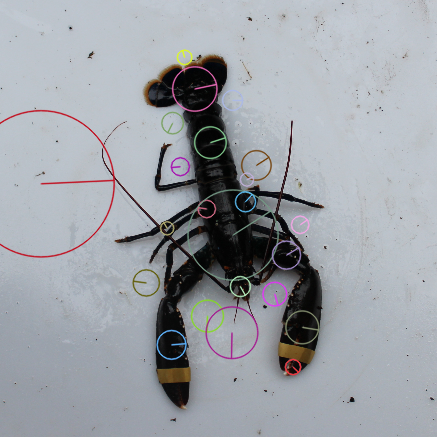
\includegraphics[width=1\textwidth, keepaspectratio]{imgs/octave.png}
\caption{Octave filtering method}
\end{figure}
\end{minipage}
\hspace{0.7cm}
\begin{minipage}{0.42\textwidth}
\begin{figure}
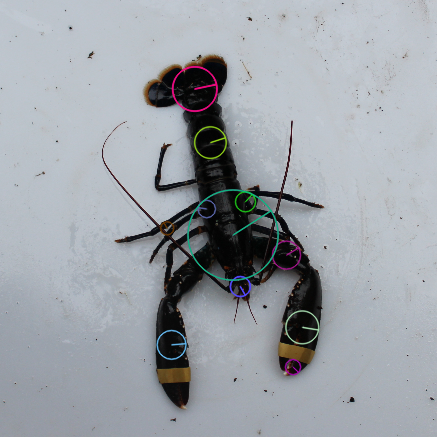
\includegraphics[width=1\textwidth, keepaspectratio]{imgs/hist.png}
\caption{Colour histogram filtering method}
\end{figure}
\end{minipage}
\end{center}
\vspace*{-0.5cm}
\end{myblock}


\begin{myblock}{Matched lobster graph}
Applying subgraph matching with probabilistic models returns the most probable subgraphs found in the image, which are combined into the final graph.
\begin{figure}
\centering
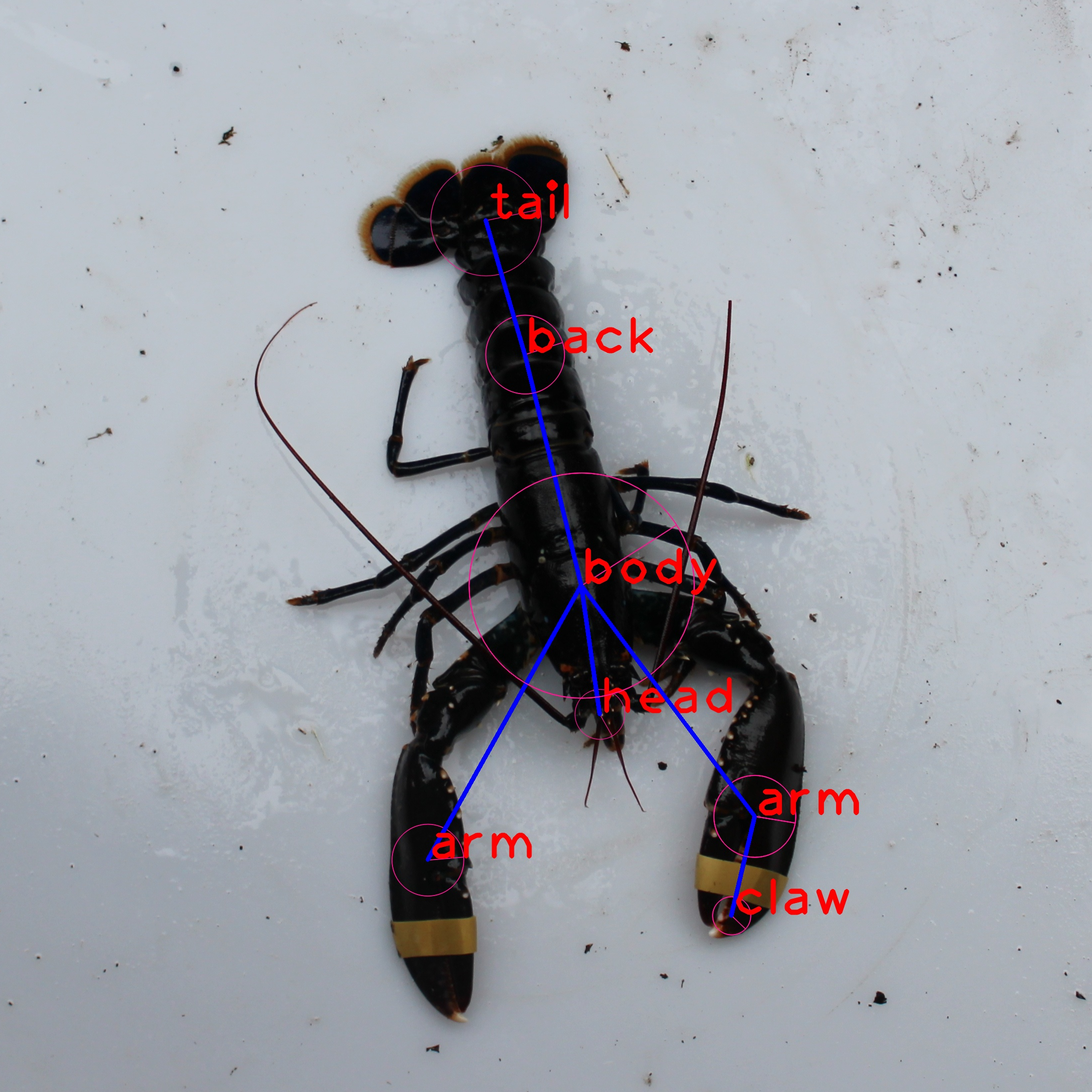
\includegraphics[width=0.7\textwidth, keepaspectratio]{imgs/matched.png}
\caption{Final matched graph drawn on top of lobster image}
\end{figure}

\end{myblock}


}\end{minipage}
\end{beamercolorbox}
\end{column}

% Right columns
\begin{column}{.57\textwidth}
\begin{beamercolorbox}[center]{postercolumn}
\begin{minipage}{.98\textwidth} % tweaks the width, makes a new \textwidth
\parbox[t][\columnheight]{\textwidth}{ % must be some better way to set the the height, width and textwidth simultaneously


\begin{myblock}{Method pipeline}
\vspace{0.2cm}
\begin{center}
\begin{minipage}{0.9\textwidth}
\centering
\begin{figure}[H]
\centering
\begin{subfigure}{\textwidth}
\centering
\begin{tikzpicture}
\node (raw) [data] {Raw lobster image};
\node (detection) [process, right of=raw, xshift=3cm] {Keypoint detection};
\node (filter) [process, right of=detection, xshift=3cm] {Keypoint filtering};
\node (creation) [process, right of=filter, xshift=3cm] {Subgraph creation};
\node (subgraph) [data, right of=creation, xshift=3cm] {Lobster subgraphs};

\draw [arrow] (raw) -- (detection);
\draw [arrow] (detection) -- (filter);
\draw [arrow] (filter) -- (creation);
\draw [arrow] (creation) -- (subgraph);

\end{tikzpicture}
\caption{Initial process of creating labelled subgraphs for matching.}
\vspace{0.5cm}
\end{subfigure}

\begin{subfigure}{\textwidth}
\centering
\begin{tikzpicture}
\node (subgraph) [data] {Lobster subgraphs};
\node (graphgrep) [process, right of=subgraph, xshift=3cm] {Subgraph matching};
\node (model) [process, right of=graphgrep, xshift=3cm] {Graph building};
\node (graph) [data, right of=model, xshift=3cm] {Matched lobster graph};

\draw [arrow] (subgraph) -- (graphgrep);
\draw [arrow] (graphgrep) -- (model);
\draw [arrow] (model) -- (graph);
\end{tikzpicture}
\caption{Process of taking the labelled subgraphs to creating a full lobster graph.}
\end{subfigure}
\caption{Flow chart of the whole matching process from getting keypoints to creation of the lobster graphs. Blue steps represent processes and red steps represent inputs and outputs.}
\label{fig:overview}
\end{figure}
\end{minipage}
\end{center}
\end{myblock}

\begin{myblock}{Probabilistic models}
A na\"{i}ve Bayes probability model was used to calculate the probability of a matched graph with $n$ nodes and $m$ edges for both the subgraph creation and graph building stages.
\vspace{-0.4cm}
\begin{align}
\begin{split}
P(\text{subgraph}) &= \prod_{i=0}^n P(\text{node}_{i}) \cdot \prod_{j=0}^m P(\text{edge}_{j})
\end{split}
\\
\begin{split}
P(\text{node}) &= P(\text{node.label}\ |\ \text{node.size})
\end{split}
\\[10pt]
\begin{split}
P(\text{edge}) &= P(\text{edge.length}\ |\ n_{1} \wedge n_{2}) \\
 &= \frac{P(n_{1} \wedge n_{2}\ |\ \text{edge.length}) \cdot P(\text{edge.length})}{P(n_{1}) \cdot P(n_{2})}
\end{split}
\end{align}

\end{myblock}

\begin{myblock}{F1 score}
The F1 score was used to determine optimal thresholds for matching and the general performance of the various methods.

\begin{minipage}{0.9\textwidth}
%\centering
\begin{figure}[H]
\centering
\begin{minipage}{0.48\textwidth}
\foneidentgraph{mature}{0.5}{legend:fone}
\end{minipage}
\hspace*{\fill}
\begin{minipage}{0.48\textwidth}
\foneidentgraph{juvenile}{0.5}{legend:fone}
\end{minipage}
\hspace*{\fill}\ref{legend:fone}
\caption{Comparison of F1 score for mature and juvenile models on all lobsters with a histogram filter threshold of 0.5}
\end{figure}
\end{minipage}

\end{myblock}


\begin{myblock}{Classification results}
A juvenile and mature model graph was developed and matched to each image in the dataset. The image is classified based on which model was better matched.
\begin{figure}[H]
\centering
\doublebargraph{legend:classification}
\ref{legend:classification}
\caption{Detailed classification results on the specific lobster categories}
\end{figure}


\end{myblock}\vfill


}\end{minipage}
\end{beamercolorbox}
\end{column}

\end{columns}
\end{frame}
\end{document}